\documentclass[../xlapes02]{subfiles}
\begin{document}

    \chapter{Reinforcement Learning Algorithms}\label{ch:reinforcement-learning-algorithms}
    In this appendix, we present pseudocode for various RL methods and algorithms, which are used in the field of RL research and applications.


    \section{Value Iteration Algorithm in DP}\label{sec:value-iteration-algorithm-in-dp}
    \begin{algorithm}[H]
        \label{alg:value-iteration}
        \SetAlgoLined
        \textbf{Value Iteration Algorithm}\\
        \textbf{Algorithm parameter:} a small threshold $\epsilon > 0$ determining accuracy of estimation\\
        \textbf{Initialize} $V(s)$, for all $s \in S$, arbitrarily except that $V(\text{terminal}) = 0$\\
        \textbf{Loop:}\\
        \quad \textbf{for each} $s \in S:$\\
        \quad \quad $v \leftarrow V(s)$\\
        \quad \quad $V(s) \leftarrow \max_a \sum_{s', r} p(s', r|s, a)(r + \gamma V(s'))$\\
        \quad \quad $\delta \leftarrow \max(\delta, |v - V(s)|)$\\
        \textbf{until} $\delta < \epsilon$\\
        \textbf{Output} a deterministic policy $\pi$, such that\\
        $\pi(s) \leftarrow \argmax_a \sum_{s', r} p(s', r|s, a)(r + \gamma V(s'))$\\
    \end{algorithm}


    \section{Q-Learning Off-policy TD Control}\label{sec:q-learning-off-policy-td-control}
    \begin{algorithm}[H]
        \caption{Q-learning (Off-policy TD Control)}
        \label{alg:q_learning}

        \textbf{Algorithm parameters:} step size $\alpha \in (0, 1]$, small $\epsilon > 0$

        Initialize $Q(s, a)$ for all $s \in \mathcal{S}^+, a \in \mathcal{A}(s)$ arbitrarily, except that $Q(\text{terminal}, \cdot) = 0$

        \textbf{Loop for each episode:}
        \For{each episode}{
            Initialize $S$
            \textbf{Loop for each step of episode:}
            \While{$S$ is not terminal}{
                Choose $A$ from $S$ using policy derived from $Q$ (e.g., $\epsilon$-greedy)
                Take action $A$, observe $R$, $S'$
                $Q(S, A) \leftarrow Q(S, A) + \alpha \cdot \left[R + \max_a Q(S', a) - Q(S, A)\right]$
                $S \leftarrow S'$
            }
        }
    \end{algorithm}


    \section{REINFORCE: Monte-Carlo Policy-Gradient Control}\label{sec:reinforce:-monte-carlo-policy-gradient-control}
    \begin{algorithm}[H]
        \SetKwComment{Comment}{/* }{ */}
        \caption{REINFORCE Algorithm}
        \label{alg:REINFORCE}

        \Comment{Input:}
        a differentiable policy parameterization $\pi(a|s, \bm{\theta})$\;
        a differentiable state-value parameterization $\hat{v}(a|\bm{w})$\;
        Algorithm parameters: step size $\alpha_{\bm{\theta}} > 0$, $\alpha_{\bm{w}} > 0$\;
        Initialize policy parameter $\bm{\theta} \in \mathbb{R}^{d'}$ and state-value weights $\bm{w} \in \mathbb{R}^{d}$ arbitrarily (e.g., $\bm{\theta} = \bm{0}, \bm{w} = \bm{0}$)\;

        \While{Loop forever (for each episode):}{
            Generate an episode $S_0, A_0, R_1, \ldots , S_T-1, A_T-1, R_T$, following $\pi(\cdot|\cdot, \theta)$\;
            \For{Loop for each step of the episode $t=0,1,\ldots,T-1$:}{
                $G_t\leftarrow\sum_{k=t+1}^{T}R_k$\;
                $\delta\leftarrow G-\hat{v}(S_t,\bm{w})$\;
                $\bm{w}\leftarrow\bm{w}+\alpha^{\bm{w}}\delta\nabla\hat{v}(S_t,\bm{w})$\;
                $\theta\leftarrow\bm{\theta}+\alpha^{\bm{\theta}}\gamma^{t}\delta\nabla \ln\pi(A_t|S_t,\bm{\theta})$\;
            }
        }
    \end{algorithm}


    %! suppress = TooLargeSection


    \chapter{Setting up and running the program}\label{ch:setting-up-and-running-the-program}
    The root directory of the thesis code contains a \texttt{README.md} file that provides instructions for installing the program.\ Following the steps outlined in this file should be sufficient for completing the installation process.

    The program has been tested on both MacOS 13.2.1 and Ubuntu 20.04.6 LTS (GNU/Linux 5.4.0-146-generic x86\_64), using Python version 3.10.11.


    \section{Prepare Environment}\label{sec:prepare-environment}
    Run these commands from the root directory of the thesis code.\ It will create a virtual environment and install the required packages:
    \begin{lstlisting}[language=bash,label={lst:prepare-environment}]
mkdir -p out/baseline out/dataset out/model # create directories for results
python3 -m venv venv # create virtual environment
source venv/bin/activate # activate virtual environment
pip3 install -r requirements.txt # install required packages
    \end{lstlisting}


    \section{Datasets}\label{sec:datasets2}
    Datasets are available at the following links:
    \begin{enumerate}
        \item \url{https://wandb.ai/investai/portfolio-allocation/artifacts/dataset/stockcombineddailydataset/v0/files}
        \item \url{https://wandb.ai/investai/portfolio-allocation/artifacts/dataset/stockfadailydataset/v2/files}
        \item \url{https://wandb.ai/investai/portfolio-allocation/artifacts/dataset/stocktadailydataset/v0/files}.
    \end{enumerate}
    Please download them and place them in the \texttt{out/dataset} folder.


    \section{Baseline}\label{sec:baseline}
    The baseline is available at the following link:
    \begin{enumerate}
        \item \url{https://wandb.ai/investai/portfolio-allocation/artifacts/baseline/baseline/v1/files}
    \end{enumerate}
    Please download it and place it in the \texttt{out/baseline} folder.


    \section{Examples of running Train/Test program}\label{sec:examples-of-running-train/test-program}
    All examples assume that the current working directory is the root directory of the thesis code.

    \subsection{\texttt{.env} file}\label{subsec:texttt{.env}-file}
    The scripts expect the \emph{.env} file in the root directory of the thesis code.\ This file contains the following variables, please fill the \texttt{WANDB\_API\_KEY} with your API key:
    \begin{lstlisting}[language=bash,label={lst:env-file}]
# W&B
WANDB_API_KEY=''
WANDB_ENTITY='investai'
WANDB_PROJECT='portfolio-allocation'
WANDB_TAGS='["None"]'
WANDB_JOB_TYPE='train'
WANDB_RUN_GROUP='exp-1'
WANDB_MODE='online'
WANDB_DIR='${PWD}/out/model'
    \end{lstlisting}
    If you don't want to use Weights \& Biases, you can remove the arguments with prefix \texttt{--wandb} from the examples (sweep run will not work), if you want to use it, it will be necessary to run the following command before running any of the following commands:
    \begin{lstlisting}[language=bash,label={lst:wandb-login}]
wandb login # to login to your W&B account
    \end{lstlisting}

    \subsection{Run the program to print the help message}\label{subsec:run-the-program-to-print-the-help-message}
    \begin{lstlisting}[language=bash,label={lst:help}]
PYTHONPATH=$PWD/investai python3 \
    investai/run/portfolio_allocation/thesis/train.py \
        --help
    \end{lstlisting}

    \subsection{Single Run (train/test)}\label{subsec:single-run-(train/test)}
    \begin{lstlisting}[language=bash,label={lst:run-train}]
PYTHONPATH=$PWD/investai python3 \
    investai/run/portfolio_allocation/thesis/train.py \
    --dataset-paths out/dataset/stockfadailydataset.csv \
    --algorithms ppo \
    --project-verbose='i' \
    --train-verbose=1 \
    --total-timesteps=1000 \
    --train=1 \
    --test=1 \
    --env-id=1 \
    --wandb=1 \
    --wandb-run-group="exp-run-1" \
    --wandb-verbose=1 \
    --baseline-path=out/baseline/baseline.csv
    \end{lstlisting}

    \subsection{Sweep Run: 3 runs with random hyperparameters over 2 datasets and 5 algorithms (train/test)}\label{subsec:sweep-run:-3-runs-with-random-hyperparameters-over-2-datasets-and-5-algorithms-(train/test)}
    \begin{lstlisting}[language=bash,label={lst:sweep-train}]
PYTHONPATH=$PWD/investai python3 \
    investai/run/portfolio_allocation/thesis/train.py \
    --dataset-paths \
        out/dataset/stockfadailydataset.csv \
        out/dataset/stockcombineddailydataset.csv \
    --algorithms \
        ppo \
        a2c \
        td3 \
        ddpg \
        sac \
    --project-verbose='i' \
    --train-verbose=1 \
    --total-timesteps=1000 \
    --train=1 \
    --test=1 \
    --env-id=1 \
    --wandb=1 \
    --wandb-sweep=1 \
    --wandb-sweep-count=3 \
    --wandb-verbose=1 \
    --wandb-run-group="exp-sweep-1" \
    --baseline-path=out/baseline/baseline.csv
    \end{lstlisting}


    \chapter{Graphs}\label{ch:graphs}


    \section{Hyperparameters Tuning Results}\label{sec:hyperparameters-tuning-results}
    \begin{figure}[H]
        \centering
        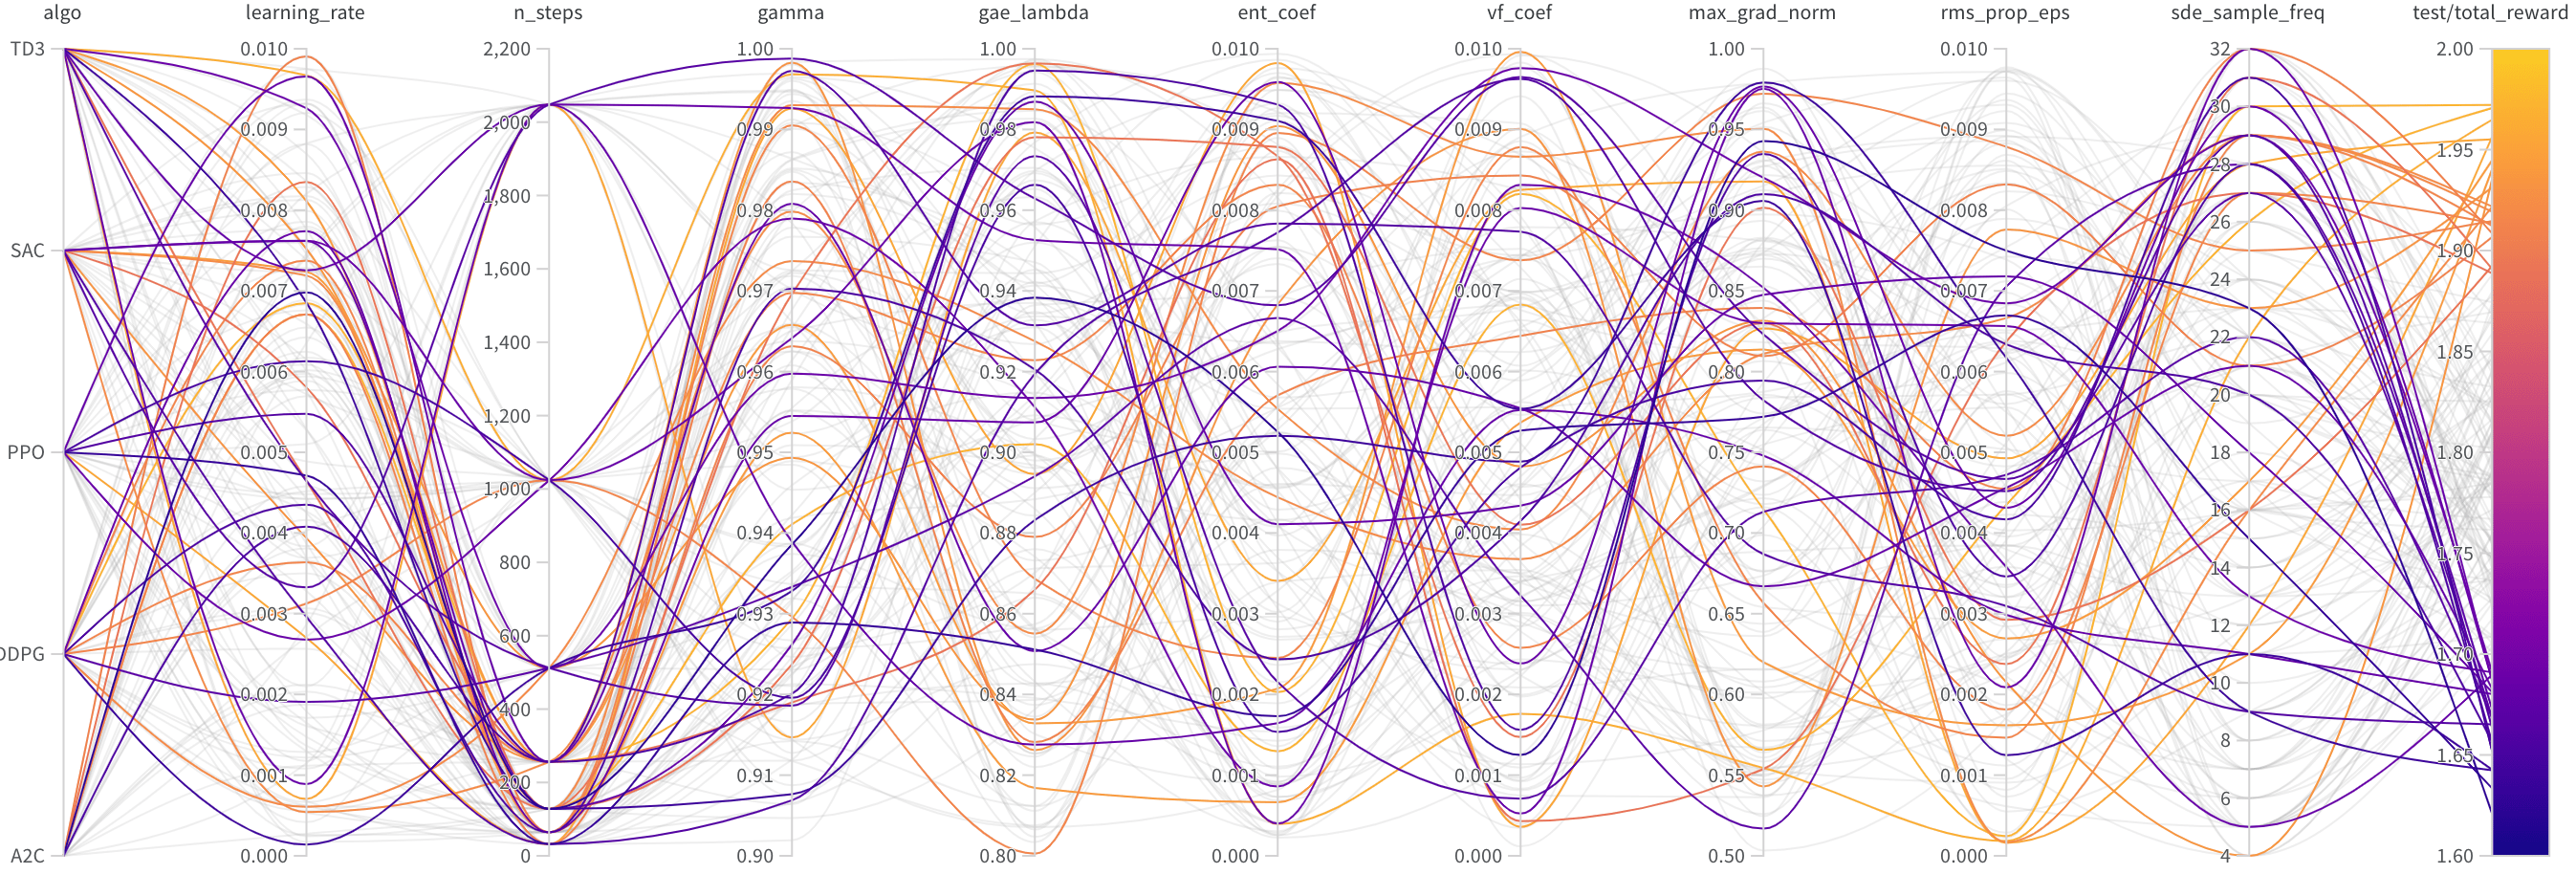
\includegraphics[width=\linewidth]{image/wandb/wb1}
        \caption{W\&B Chart of parameters and their performance}
        \label{fig:wb-chart1}
    \end{figure}

    \begin{figure}[H]
        \centering
        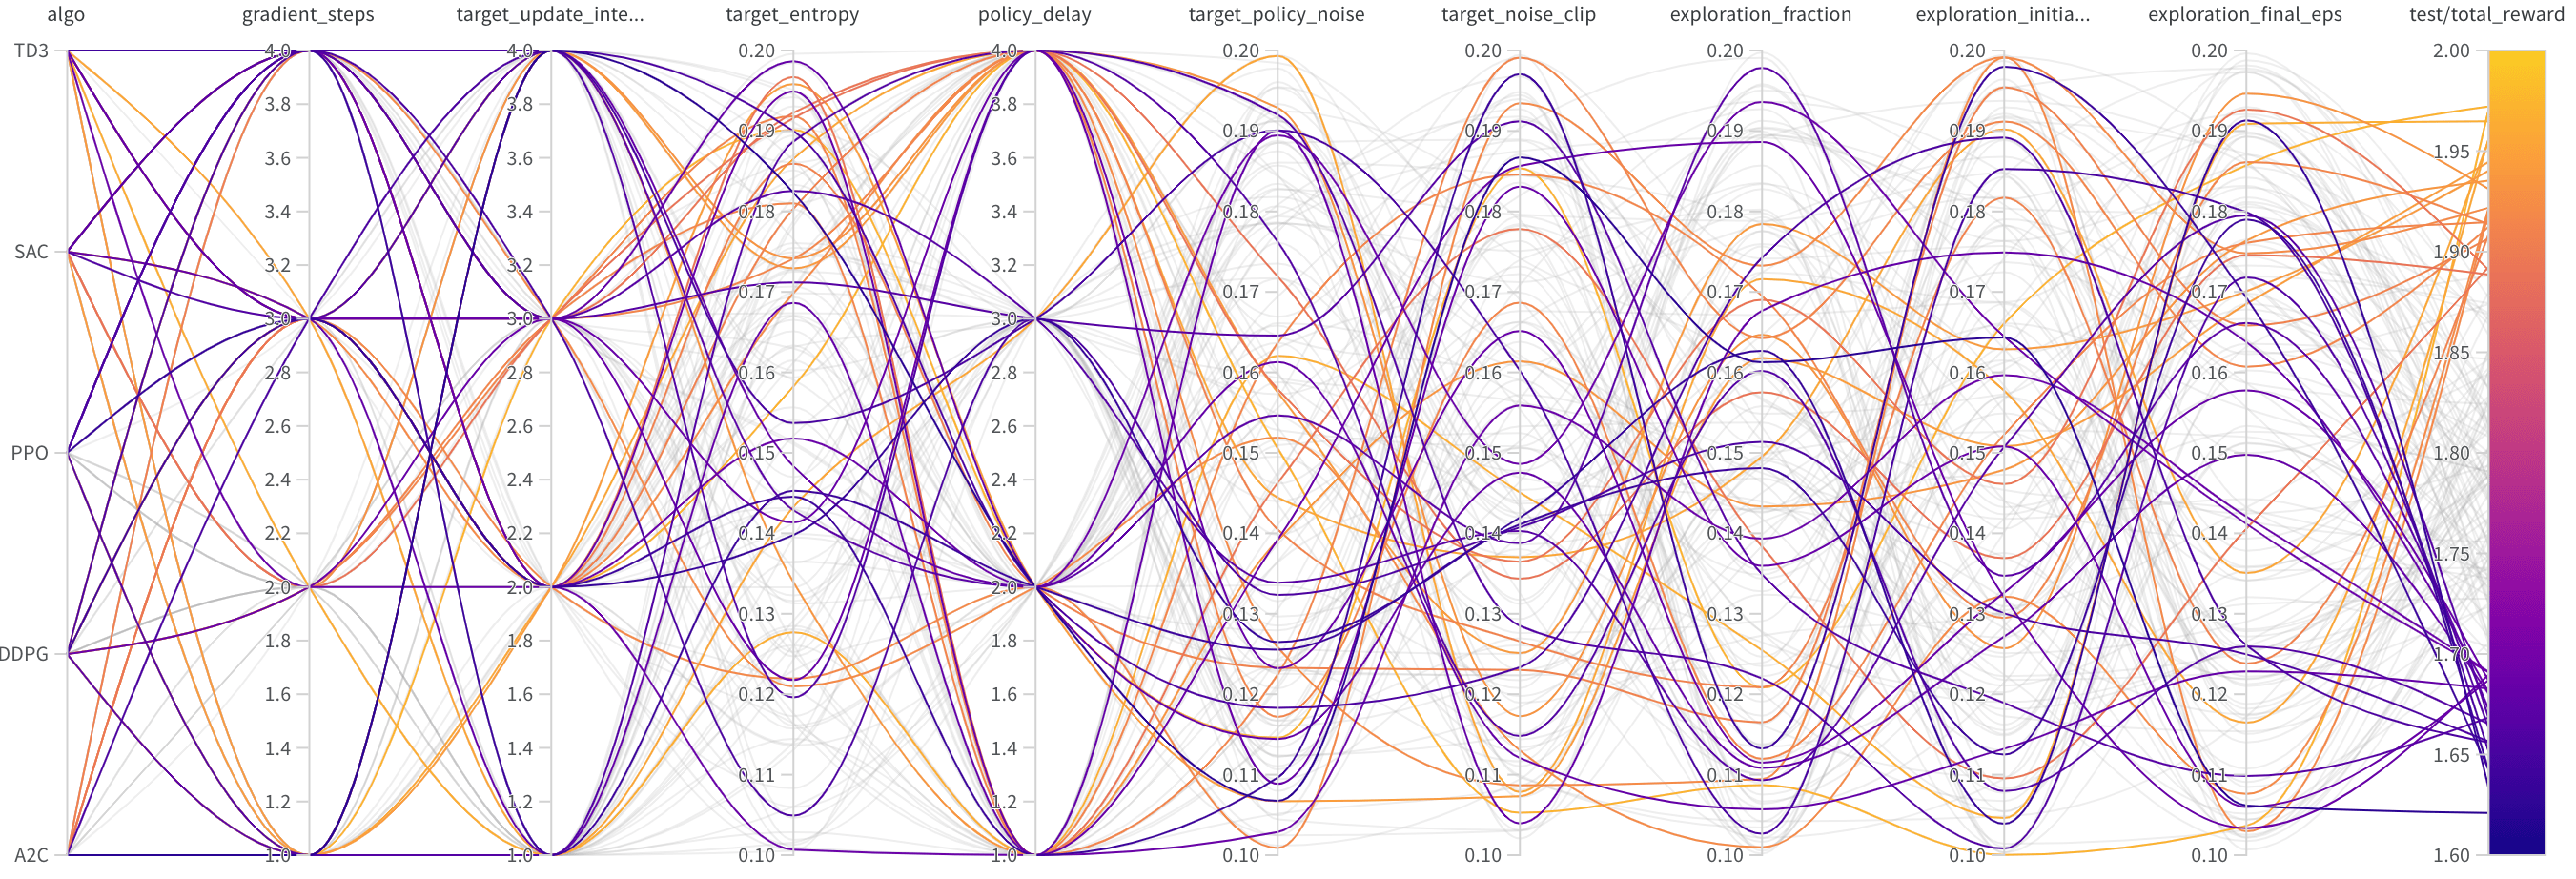
\includegraphics[width=\linewidth]{image/wandb/wb2}
        \caption{W\&B Chart of parameters and their performance}
        \label{fig:wb-chart2}
    \end{figure}

    \begin{figure}[H]
        \centering
        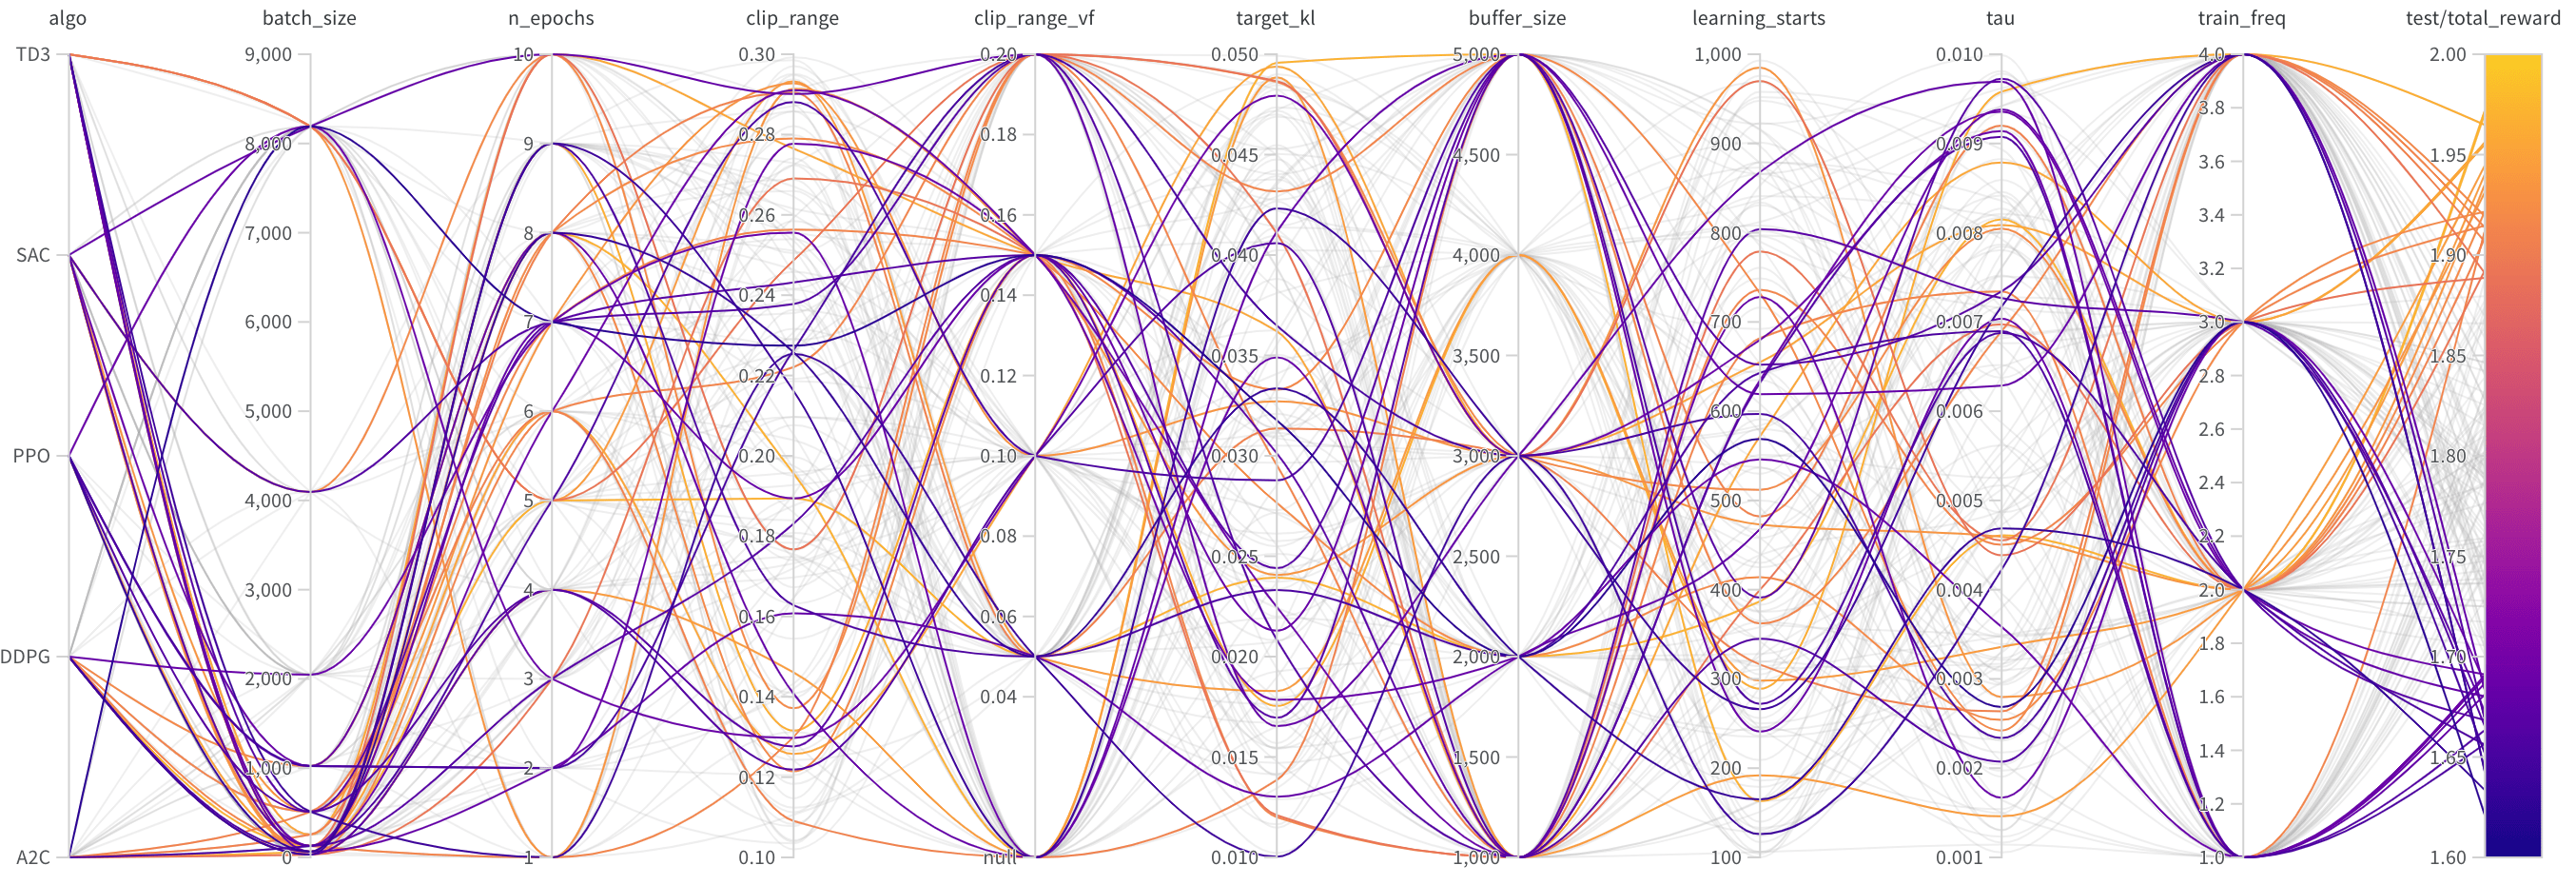
\includegraphics[width=\linewidth]{image/wandb/wb3}
        \caption{W\&B Chart of parameters and their performance}
        \label{fig:wb-chart3}
    \end{figure}

\end{document}
